\chapter{Desenvolvimento do experimento}

Nesse capítulo é apresentado o desenvolvimento do experimento, baseado nos conceitos apresentados nos capítulos anteriores. Em especial, esse capítulo mostra como as ferramentas do capítulo \ref{chap:prop} (\nameref{chap:prop}) foram utilizadas para a comparação dos resultados dos algoritmos apresentados no capítulo \ref{chap:ais} (\nameref{chap:ais}).

\section{Preparação dos dados}

Os dois conjuntos de dados utilizados (\emph{cr.ger} e \emph{cr.aust}) se encontravam em formato de texto, com os atributos separados por espaços e as instâncias separadas pelo caractere nova linha. As listagens \ref{lst:dev_data_ger} e \ref{lst:dev_data_aust} mostram as instâncias dos conjuntos de dados no formato do arquivo original (a primeira coluna representa o número da linha, e não faz parte dos dados)\footnote{Aqui são mostradas apenas as primeiras cinco instâncias dos conjuntos de dados \emph{Cr.Ger} e \emph{Cr.Aust}. Eles possuem 1000 e 650 instâncias, respectivamente}.

\vspace{0.5cm}
\begin{lstlisting}[caption=Formato original dos dados (\emph{Cr.Ger}), label=lst:dev_data_ger]
A11 6 A34 A43 1169 A65 A75 4 A93 A101 4 A121 67 A143 A152 2 A173 1 A192 A201 1
A12 48 A32 A43 5951 A61 A73 2 A92 A101 2 A121 22 A143 A152 1 A173 1 A191 A201 2
A14 12 A34 A46 2096 A61 A74 2 A93 A101 3 A121 49 A143 A152 1 A172 2 A191 A201 1
A11 42 A32 A42 7882 A61 A74 2 A93 A103 4 A122 45 A143 A153 1 A173 2 A191 A201 1
A11 24 A33 A40 4870 A61 A73 3 A93 A101 4 A124 53 A143 A153 2 A173 2 A191 A201 2
\end{lstlisting}
\vspace{0.5cm}

\vspace{0.5cm}
\begin{lstlisting}[caption=Formato original dos dados (\emph{Cr.Aust}), label=lst:dev_data_aust]
1 22.08 11.46 2 4 4 1.585 0 0 0 1 2 100 1213 0
0 22.67 7 2 8 4 0.165 0 0 0 0 2 160 1 0
0 29.58 1.75 1 4 4 1.25 0 0 0 1 2 280 1 0
0 21.67 11.5 1 5 3 0 1 1 11 1 2 0 1 1
1 20.17 8.17 2 6 4 1.96 1 1 14 0 2 60 159 1
\end{lstlisting}
\vspace{0.5cm}

A preparação dos dados para a importação no WEKA consistiu na adição de uma seção de cabeçalho e da formatação dos dados para valores separados por vírgula (seção \ref{sec:prop_arff}) e o resultado é mostrado nas listagens \ref{lst:dev_arff_ger} e \ref{lst:dev_arff_aust} (essas listagens mostram apenas as primeiras cinco instâncias na seção de dados).

\vspace{0.5cm}
\begin{lstlisting}[caption=Arquivo ARFF do \emph{Cr.Ger}, label=lst:dev_arff_ger]
@relation cr.ger

@attribute A1  {A11,A12,A13,A14}
@attribute A2  numeric
@attribute A3  {A30,A31,A32,A33,A34}
@attribute A4  {A40,A41,A42,A43,A44,A45,A46,A47,A48,A49,A410}
@attribute A5  numeric
@attribute A6  {A61,A62,A63,A64,A65}
@attribute A7  {A71,A72,A73,A74,A75}
@attribute A8  numeric
@attribute A9  {A91,A92,A93,A94,A95}
@attribute A10 {A101,A102,A103}
@attribute A11 numeric
@attribute A12 {A121,A122,A123,A124}
@attribute A13 numeric
@attribute A14 {A141,A142,A143}
@attribute A15 {A151,A152,A153}
@attribute A16 numeric
@attribute A17 {A171,A172,A173,A174}
@attribute A18 numeric
@attribute A19 {A191,A192}
@attribute A20 {A201,A202}
@attribute A21 {1,2}

@data
A11,6,A34,A43,1169,A65,A75,4,A93,A101,4,A121,67,A143,A152,2,A173,1,A192,A201,1
A12,48,A32,A43,5951,A61,A73,2,A92,A101,2,A121,22,A143,A152,1,A173,1,A191,A201,2
A14,12,A34,A46,2096,A61,A74,2,A93,A101,3,A121,49,A143,A152,1,A172,2,A191,A201,1
A11,42,A32,A42,7882,A61,A74,2,A93,A103,4,A122,45,A143,A153,1,A173,2,A191,A201,1
A11,24,A33,A40,4870,A61,A73,3,A93,A101,4,A124,53,A143,A153,2,A173,2,A191,A201,2
\end{lstlisting}
\vspace{0.5cm}

\vspace{0.5cm}
\begin{lstlisting}[caption=Arquivo ARFF do \emph{Cr.Aust}, label=lst:dev_arff_aust]
@relation cr.aust

@attribute A1  {0,1}
@attribute A2  numeric
@attribute A3  numeric
@attribute A4  {1,2,3}
@attribute A5  {1,2,3,4,5,6,7,8,9,10,11,12,13,14}
@attribute A6  {1,2,3,4,5,6,7,8,9}
@attribute A7  numeric
@attribute A8  {1,0}
@attribute A9  {1,0}
@attribute A10 numeric
@attribute A11 {1,0}
@attribute A12 {1,2,3}
@attribute A13 numeric
@attribute A14 numeric
@attribute A15 {0,1}

@data
1,22.08,11.46,2,4,4,1.585,0,0,0,1,2,100,1213,0
0,22.67,7,2,8,4,0.165,0,0,0,0,2,160,1,0
0,29.58,1.75,1,4,4,1.25,0,0,0,1,2,280,1,0
0,21.67,11.5,1,5,3,0,1,1,11,1,2,0,1,1
1,20.17,8.17,2,6,4,1.96,1,1,14,0,2,60,159,1
\end{lstlisting}
\vspace{0.5cm}

Com os arquivos no formato ARFF, os conjuntos de dados podem ser importados no WEKA. A figura \ref{fig:dev_weka_arff} mostra o conjunto de dados \emph{Cr.Ger} quando importado. Um conjunto de dados importado pode ser utilizado para qualquer algoritmo que suporte os tipos de atributos contidos nele.

\vspace{0.5cm}
\begin{figure}[h!]
    \centering
    \caption{Conjunto de dados \emph{Cr.Ger importado no WEKA}}
    \label{fig:dev_weka_arff}
    \vspace{0.5cm}
    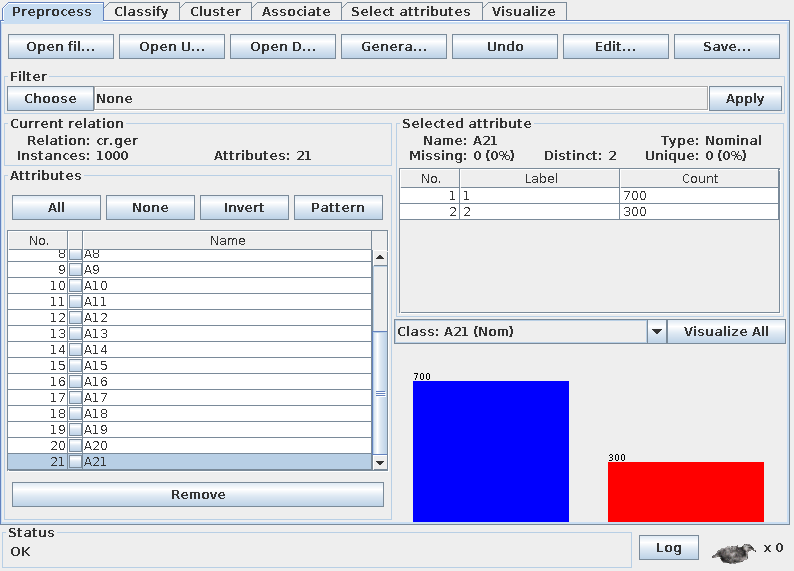
\includegraphics[width=0.75\textwidth]{img/cr_ger.png}
    \vspace{0.5cm}
\end{figure}
\vspace{0.5cm}

\section{Utilizando o WEKA}

O WEKA é dividido em dois módulos principais: Explorer e Experimenter. Além disso, o WEKA apresenta duas interfaces principais: linha de comando (\emph{command-line interface}, CLI\nomenclature{CLI}{Command-line Interface}) e gráfica (\emph{graphical user interface}, GUI\nomenclature{GUI}{Graphical User Interface}). A interface gráfica é mais apropriada para exploração e experimentação, e para a apresentação dos dados, algoritmos e resultados. A interface de linha de comando é mais apropriada para automatização de tarefas e integração com outros sistemas, além de consumir menos recursos. Os dois módulos podem ser usados em qualquer uma das duas interfaces, com as mesmas funcionalidades.

Nesse trabalho foi utilizado o módulo \emph{Experimenter} na interface por linha de comando. O módulo \emph{Experimenter} tem um formato de arquivo de configuração que facilita a definição de experimentos e a repetição e automação dos testes para cada algoritmo usando a interface por linha de comando é muito mais fácil do que se fosse utilizada a interface gráfica. Os exemplos de execução são apresentados conforme devem ser digitados em uma interface de linha de comando, em um emulador de terminal, utilizando um \emph{shell} como \emph{sh} ou \emph{bash}.

\subsection{Filtros}
\label{sec:dev_weka_filters}

No WEKA, um filtro é um objeto que recebe um conjunto de dados como entrada e produz um conjunto de dados modificado. Esse é um processo comum da Mineração de Dados, chamado de pré-processamento dos dados: adicionar, remover ou alterar atributos, etc.

Um filtro comum, que é utilizado nesse trabalho, é o de criação de partições para o \emph{cross-validation}. Para esse filtro, são passados três argumentos. O argumento \emph{c} indica qual dos atributos é o atributo correspondente à classe, e é representado por um índice, iniciado em 1, conforme a declaração na seção de atributos do arquivo de dados (caso o padrão do WEKA seja usado, ou seja, o atributo de classe seja o último da listagem, pode ser utilizado o valor ``\emph{last}'' como argumento). O argumento \emph{N} indica o número de partições, e o argumento \emph{F} indica o índice da partição selecionada.

Além desses, o argumento \emph{V} pode ser utilizado para gerar o conjunto inverso de seleções, útil para dividir o conjunto em duas partes complementares. Dessa forma, para gerar um conjunto de dados para testes e outro para treinamento, podem ser usados comandos como os da listagem \ref{lst:dev_filter}\footnote{Nesses exemplos, é usado o redirecionamento de entrada e saída presentes na maioria dos \emph{shells} UNIX. O caractere ``<'' seguido de um nome de arquivo indica que aquele arquivo será usado como entrada para o comando. De maneira semelhante, o caractere ``>'' seguido de um nome de arquivo indica que ele será usado como saída. O WEKA também permite que sejam utilizadas as opções \emph{i} e \emph{o}, respectivamente, para obter os mesmos resultados. No primeiro exemplo, a forma equivalente seria ``\emph{-i dataset.arff -o dataset\_test.arff}''.}. Nesse exemplo, são o conjunto de dados é dividido em quatro partições, conforme indicado pelo argumento N. Na primeira linha, a primeira partição é escolhida, conforme indicado pelo argumento F. Na segunda, todas as partições com exceção da primeira são selecionadas, conforme indicado pelo parâmetro V.

\begin{lstlisting}[caption=Filtro para geração de partições para \emph{cross-validation}, label=lst:dev_filter]
java weka.filters.supervised.instance.StratifiedRemoveFolds -c last -N 4 -F 1 \
    < dataset.arff > dataset_test.arff
java weka.filters.supervised.instance.StratifiedRemoveFolds -c last -N 4 -F 1 -V \
    < dataset.arff > dataset_train.arff
\end{lstlisting}

\subsection{Execução de um classificador}

A execução de um algoritmo é feita através da classe que implementa o algoritmo no WEKA. Diversas opções podem ser passadas na linha de comando para mudar os parâmetros do algoritmo. Existem algumas opções adicionais para especificar dados adicionais, como os arquivos de dados para treinamento e testes. Além das opções gerais, cada algoritmo pode aceitar diferentes tipo de opções específicas. Como exemplo, para gerar a saída da listagem \ref{lst:prop_weka_out}, foi utilizado o comando da listagem \ref{lst:dev_exec_classifier}.

\vspace{0.5cm}
\begin{lstlisting}[caption=Execução de um classificador, label=lst:dev_exec_classifier]
java weka.classifiers.neural.lvq.Lvq1 -t data/weather.numeric.arff -i
\end{lstlisting}
\vspace{0.5cm}

Como é possível ver, a linha de comando é reproduzida no atributo ``\emph{Scheme}'' na saída. Esse atributo pode ser consultado para executar exatamente o mesmo teste novamente, tornando a reprodução do experimento muito mais fácil. As diversas opções do atributo que não estão presentes na linha de comando são os parâmetros do algoritmo. Como não foram especificados na linha de comando, foram assumidos os valores padrão, que são mostrados na saída. As duas opções que não estão presentes na saída são a opção ``\emph{i}'', que mostra uma saída mais completa e a opção ``\emph{t}'', que indica o arquivo que será utilizado como entrada.

Para executar os algoritmos do pacote de algoritmos imunológicos, é necessário informar à máquina virtual a localização do arquivo que contém o código executável. Esse código é disponibilizado em um arquivo \emph{jar}, um tipo de arquivo específico da linguagem java que é semelhante a um arquivo compactado utilizando os programas \emph{tar} ou \emph{zip}.

Para indicar o arquivo, é utilizada a opção \emph{classpath} da máquina virtual. Essa opção pode ser utilizada tanto para indicar um diretório contendo os arquivos compilados (arquivos \emph{.class}) quanto um arquivo \emph{jar}. Alternativamente, o arquivo \emph{jar} pode ser descompactado e o diretório gerado utilizado. Essa opção pode ser passada na linha de comando ou como uma variável de ambiente. Para executar o algoritmo AIRS, por exemplo, é utilizado qualquer um dos comandos da listagem \ref{lst:dev_weka_airs}. A sintaxe da opção \emph{classpath} é semelhante ao \emph{path} da maioria dos sistemas operacionais, ou seja, uma lista dos caminhos e arquivos separados pelo caractere ``:'' (dois-pontos) em sistemas Unix ou ``;'' (ponto-e-vírgula) em sistemas Windows.

\vspace{0.5cm}
\begin{lstlisting}[caption=Execução de um algoritmo do pacote de algoritmos imunológicos, label=lst:dev_weka_airs]
# Opção na linha de comando.
java -classpath wekaclassalgos.jar weka.classifiers.immune.airs.AIRS1 # parâmetros
# Variável de ambiente.
CLASSPATH=wekaclassalgos.jar
java weka.classifiers.immune.airs.AIRS1 # parâmetros
\end{lstlisting}
\vspace{0.5cm}

Combinando os conceitos apresentados nessa seção, a execução de um teste para um algoritmo imunológico utilizando um dos conjuntos de dados é feita de acordo com a listagem \ref{lst:dev_weka_single}. Aqui, é usado a opção ``\emph{t}'' para especificar o conjunto de dados \emph{Cr.Ger}. Todas as outras opções são parâmetros do filtro (os valores utilizados são os valores padrão para esse algoritmo).

\vspace{0.5cm}
\begin{lstlisting}[caption=Execução de um algoritmo do pacote de algoritmos imunológicos utilizando um dos conjuntos de dados, label=lst:dev_weka_single]
# Variável de ambiente.
CLASSPATH=wekaclassalgos.jar
java weka.classifiers.immune.airs.AIRS1 \
    -S 1 -F 0.2 -C 10.0 -H 2.0 -M 0.1 -R 150.0 -V 0.9 -A -1 -B 1 -E 1 -K 3 \
    -t german.arff
\end{lstlisting}
\vspace{0.5cm}

\subsection{Execução dos classificadores}

Para a execução de um teste, pode ser criado um executor genérico de classificadores, com base na listagem \ref{lst:dev_weka_template}:

\vspace{0.5cm}
\begin{lstlisting}[caption=Execução genérica de um classificador, label=lst:dev_weka_template]
# Variável de ambiente.
java -classpath "$classpath" \
    "$classificador" "$parametros" -t "$conjunto_de_dados" \
    > "$arquivo_resultados"
\end{lstlisting}
\vspace{0.5cm}

Dessa forma, é possível utilizar o mesmo comando para execução, variando apenas os valores das variáveis. Os valores utilizados para cada variável foram:

\begin{enumerate}[a)]
    \item \emph{classpath}: conforme explicado na sessão anterior. Esse valor não muda entre as execuções dos testes, mas é mantido como uma variável para que ele possa ser facilmente alterado caso necessário. Esse é o arquivo \emph{jar} do WEKA que contém a implementação dos algoritmos imunológicos (\emph{wekaclassalgos.jar}). Esse arquivo também contém os algoritmos do WEKA, então ele é a única dependência necessária para utilizar os classificadores imunológicos e os que já são incluídos no WEKA.
    \item \emph{classificador}: todos os classificadores testados no experimento:
        \begin{enumerate}[a)]
            \item weka.classifiers.immune.airs.AIRS2
            \item weka.classifiers.immune.immunos.Immunos99
            \item weka.classifiers.immune.clonalg.CLONALG
            \item weka.classifiers.functions.MultilayerPerceptron
            \item weka.classifier.functions.SMO
            \item weka.classifiers.meta.AttributeSelectedClassifier
            \item weka.classifiers.trees.J48
            \item weka.classifiers.neural.lvq.Lvq2\_1
        \end{enumerate}
    \item \emph{parâmetros}: os parâmetros são listados junto com cada classificador no arquivo de configuração.
    \item \emph{conjunto\_de\_dados}: o caminho para o arquivo ARFF dos dois conjuntos de dados utilizados.
    \item \emph{arquivo\_resultados}: arquivo onde os resultados são gravados.
\end{enumerate}

\subsection{Seleção de parâmetros no WEKA}

Conforme descrito no capítulo \ref{chap:eval}, o desempenho de um algoritmo depende da escolha dos parâmetros utilizados. Como o processo de escolha de parâmetros é repetitivo e fácil de ser automatizado, existem métodos para escolher os parâmetros que geram o melhor valor para os parâmetros de um modelo para um conjunto de dados específico. Um desses métodos, muito utilizado por sua simplicidade e eficácia (embora não seja tão eficiente), é o \emph{grid search}.

No WEKA, existem duas implementações desse método. Ambos fazem parte de uma categoria denominada \emph{meta-classificadores}\footnote{Esses e outros meta-classificadores que o WEKA disponibiliza podem ser encontrados no pacote \emph{weka.classifiers.meta}.}, ou seja, classificadores que atuam sobre a execução de outros classificadores. Esses dois componentes são \emph{GridSearch} e \emph{CVParameterSelection}, e seu funcionamento é semelhante. O processo para utilizá-los para a escolha de parâmetros é o seguinte:

\begin{enumerate}[a)]
    \item Indicar o meta-classificador utilizado.
    \item Indicar o classificador real que será utilizado.
    \item Listar os parâmetros que serão testados.
    \item Listar a faixa de valores para os parâmetros.
    \item Indicar o conjunto de dados que será utilizado.
    \item Executar o teste.
\end{enumerate}

Com exceção dos itens \emph{a)} e \emph{d)}, o processo é semelhante à execução de um classificador comum. De fato, o meta-classificador executará o classificador da mesma forma que o WEKA faria. No entanto, ao invés de um única execução com parâmetros fixos, esses dois meta-classificadores fazem diversos testes, utilizando todas as combinações possíveis dos valores listados no item \emph{d)} para os parâmetros.

É importante levar em consideração que, conforme discutido anteriormente, esse processo é de grande utilidade para determinar os melhores valores para os parâmetros do classificador, no entanto, uma óbvia desvantagem é o grande aumento no tempo de execução. O número de combinações possíveis cresce exponencialmente com o número de parâmetros e número de elementos na faixa de valores para esses parâmetros.

Existem formas de amenizar o efeito da explosão combinatória desses métodos. A opção mais popular aproveita o grande potencial de paralelização do processo de execução do classificador com diferentes parâmetros. Como cada execução é completamente independente das outras, e podem ser executadas em paralelo. Na prática, grandes quantidades de unidades de processamento (denominados \emph{clusters}) são utilizados, e conjuntos de combinações de valores são distribuídas para cada um. Dessa forma, é possível aproveitar ao máximo a quantidade de recursos disponíveis. Os resultados dos testes podem então ser combinados em uma única unidade para a análise final.

\section{\emph{Experimenter}}

Além do módulo \emph{Explorer}, para execução de testes, o WEKA apresenta um módulo para configuração e execução de experimentos, chamado \emph{Experimenter} (figura \ref{fig:dev_weka_experimenter}). Esse módulo facilita a criação de experimentos, criando um arquivo de configuração onde são descritas as etapas, que pode ser utilizado para reproduzir o experimento usando as mesmas configurações.

\begin{figure}[h!]
\vspace{0.5cm}
    \centering
    \caption{Experimenter}
    \label{fig:dev_weka_experimenter}
    \vspace{0.5cm}
    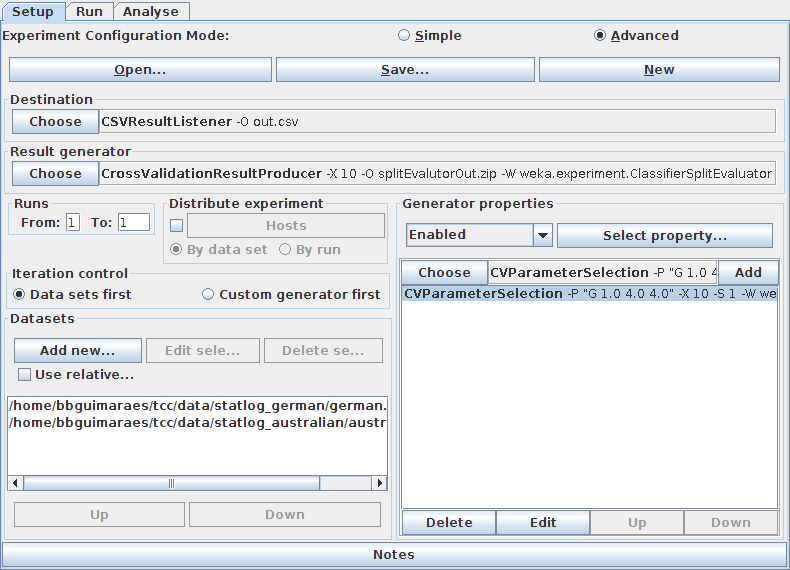
\includegraphics[width=0.75\textwidth]{img/experimenter.png}
    \vspace{0.5cm}
\vspace{0.5cm}
\end{figure}

A configuração do \emph{Experimenter} pode ser dividida nas seções:

\begin{enumerate}
    \item \textbf{Entrada}: a fonte do conjunto de dados. O padrão do WEKA é utilizar arquivos ARFF, mas todos os tipos de arquivos suportados podem ser usados, como arquivos CSV. Também é possível utilizar mais de um conjunto de dados para o mesmo experimento.
    \item \textbf{Tipo de experimento}: \emph{cross-validation} ou divisão fixa em dados de treino e teste.
    \item \textbf{Iterações}: número de execuções do experimento.
    \item \textbf{Algoritmos}: os algoritmos que serão testados. É possível configurar o parâmetros de cada algoritmo exatamente como é feito no \emph{Explorer}.
    \item \textbf{Saída}: o local onde os resultados do experimento serão gravados. O padrão é um arquivo CSV, mas outros tipos podem ser usados, com arquivos ARFF ou bancos de dados.
\end{enumerate}

Essas configurações podem ser gravadas em um arquivo para que possam ser reutilizadas. O formato desse arquivo pode ser tanto uma representação em formato binário exclusiva do WEKA ou um arquivo CSV.

A partir de um arquivo de configuração é possível executar um experimento usando a interface gráfica. Também é possível utilizar a interface de linha de comando, conforme a listagem \ref{lst:dev_run_experiment}.

\vspace{0.5cm}
\begin{lstlisting}[caption=Execução de um experimento, label=lst:dev_run_experiment]
# Flags:
#     -l: indica o arquivo de configuração (load).
#     -r: executar o experimento (run).
java weka.experiment.Experiment -l exp.xml -r
\end{lstlisting}
\vspace{0.5cm}

\subsection{Resultados}

Conforme mencionado acima, o formato padrão de gravação dos resultados de um experimento pelo \emph{Experimenter} é em arquivos CSV. É gerada uma linha no arquivo com as informações e resultados a cada execução. O número de linha gerado é igual ao número de execuções na configuração do experimento, multiplicado pelo número de \emph{folds} usado no \emph{cross-validation} (caso essa opção tenha sido selecionada), multiplicado pelo número de conjuntos de dados (que pode ser apenas um). Dessa forma, caso o número de execuções seja configurado como "10", o número de \emph{folds} como "10" e sejam utilizados dois conjuntos de dados, serão geradas 200 linhas de resultados no arquivo de saída.

Para cada execução são gravados dados sobre os resultados do treinamento e da classificação das instâncias. Esses dados são os mesmos exibidos quando uma classificação é executada usando o módulo \emph{Explorer} (listagem \ref{lst:prop_weka_out}). Uma lista completa das variáveis é mostrada na listagem \ref{lst:dev_experimenter_header}.

\vspace{0.5cm}
\begin{lstlisting}[caption=Variáveis gravados pelo \emph{Experimenter}, label=lst:dev_experimenter_header]
Key_Dataset
Key_Run
Key_Fold
Key_Scheme
Key_Scheme_options
Key_Scheme_version_ID
Date_time
Number_of_training_instances
Number_of_testing_instances
Number_correct
Number_incorrect
Number_unclassified
Percent_correct
Percent_incorrect
Percent_unclassified
Kappa_statistic
Mean_absolute_error
Root_mean_squared_error
Relative_absolute_error
Root_relative_squared_error
SF_prior_entropy
SF_scheme_entropy
SF_entropy_gain
SF_mean_prior_entropy
SF_mean_scheme_entropy
SF_mean_entropy_gain
KB_information
KB_mean_information
KB_relative_information
True_positive_rate
Num_true_positives
False_positive_rate
Num_false_positives
True_negative_rate
Num_true_negatives
False_negative_rate
Num_false_negatives
IR_precision
IR_recall
F_measure
Area_under_ROC
Weighted_avg_true_positive_rate
Weighted_avg_false_positive_rate
Weighted_avg_true_negative_rate
Weighted_avg_false_negative_rate
Weighted_avg_IR_precision
Weighted_avg_IR_recall
Weighted_avg_F_measure
Weighted_avg_area_under_ROC
Elapsed_Time_training
Elapsed_Time_testing
UserCPU_Time_training
UserCPU_Time_testing
Serialized_Model_Size
Serialized_Train_Set_Size
Serialized_Test_Set_Size
Summary
\end{lstlisting}
\vspace{0.5cm}

Essas variáveis contém informações sobre o conjunto de dados (nome e número de instâncias de treinamento e testes), classificador (nome e parâmetros), sobre o processo de treinamento e classificação (data, tempo de execução e consumo de memória) e sobre os resultados (diversas medidas de eficácia).

\section{Seleção de algoritmos}

Todos os algoritmos utilizados para comparação com os algoritmos imunológicos fazem parte da distribuição padrão do WEKA (a versão utilizada é a 3.6.9 de 25 de janeiro de 2013). A figura \ref{fig:dev_weka_algos} mostra os algoritmos na listagem de classificadores do WEKA. Os algoritmos serão descritos brevemente nas próximas seções.

\iffalse add value of default parameters \fi

\vspace{0.5cm}
\begin{figure}[h]
    \centering
    \caption{Algoritmos no WEKA}
    \label{fig:dev_weka_algos}
    \vspace{0.5cm}
    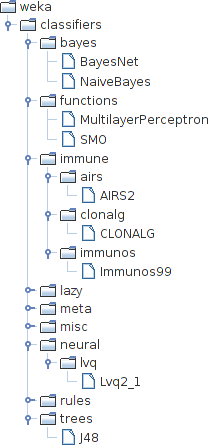
\includegraphics[height=0.5\textheight]{img/weka_algos_cropped.png}
    \vspace{0.5cm}
\end{figure}
\vspace{0.5cm}

\subsection{Redes neurais artificiais}

Um algoritmo que utiliza uma rede de neurônios artificiais inspirados no modelo dos neurônios biológicos do sistema nervoso. Simula uma rede de neurônios usando um modelo computacional baseado nas conexões entre os neurônios.

\subsubsection{MultilayerPerceptron}

Uma implementação de uma rede neural multicamadas que usa o algoritmo \emph{backpropagation}, proposto por Paul Werbos \cite{Werbos1974}. A aprendizagem acontece através de repetidas iterações e ajustes dos pesos das conexões entre neurônios. Pode ser treinada de forma automática, mas o WEKA oferece uma interface onde os pesos da rede podem ser alterados manualmente.

\begin{enumerate}[a)]
    \item \textbf{Parâmetros}:
        \begin{itemize}
            \iffalse <learning rate>. Learning Rate for the backpropagation algorithm. (Value should be between 0 - 1, Default = 0.3). \fi
            \item \textbf{L}: taxa de aprendizagem.
            \iffalse <momentum>. Momentum Rate for the backpropagation algorithm. (Value should be between 0 - 1, Default = 0.2). \fi
            \item \textbf{M}: taxa de \emph{momentum}.
            \iffalse <number of epochs>. Number of epochs to train through. (Default = 500). \fi
            \item \textbf{N}: número de \emph{epochs} (uma iteração do processo de treinamento e teste).
            \iffalse <percentage size of validation set>. Percentage size of validation set to use to terminate training (if this is non zero it can pre-empt num of epochs. (Value should be between 0 - 100, Default = 0). \fi
            \item \textbf{V}: tamanho do conjunto de validação do treinamento.
            \iffalse <seed>. The value used to seed the random number generator(Value should be >= 0 and and a long, Default = 0). \fi
            \item \textbf{S}: semente do gerador de números aleatórios.
            \iffalse <threshold for number of consequetive errors>. The consequetive number of errors allowed for validation testing before the netwrok terminates. (Value should be > 0, Default = 20). \fi
            \item \textbf{E}: número máximo de erros consecutivos para término da validação da rede.
            \iffalse GUI will be opened. (Use this to bring up a GUI). \fi
            \item \textbf{G}: abre a interface de criação da rede.
            \iffalse Autocreation of the network connections will NOT be done. (This will be ignored if -G is NOT set) \fi
            \item \textbf{A}: não cria as conexões da rede.
            \iffalse A NominalToBinary filter will NOT automatically be used. (Set this to not use a NominalToBinary filter). \fi
            \item \textbf{B}: não aplica o filtro NominalToBinary.
            \iffalse <comma seperated numbers for nodes on each layer>. The hidden layers to be created for the network. (Value should be a list of comma separated Natural numbers or the letters 'a' = (attribs + classes) / 2, 'i' = attribs, 'o' = classes, 't' = attribs .+ classes) for wildcard values, Default = a). \fi
            \item \textbf{H}: parâmetro para configuração das camadas escondidas da rede.
            \iffalse Normalizing a numeric class will NOT be done. (Set this to not normalize the class if it's numeric). \fi
            \item \textbf{C}: desabilita a aplicação de normalização no atributo de classe.
            \iffalse Normalizing the attributes will NOT be done. (Set this to not normalize the attributes). \fi
            \item \textbf{I}: desabilita a aplicação de normalização em todos os atributos.
            \iffalse Reseting the network will NOT be allowed. (Set this to not allow the network to reset). \fi
            \item \textbf{R}: desabilita a reinicialização da rede durante o treinamento.
            \iffalse Learning rate decay will occur. (Set this to cause the learning rate to decay). \fi
            \item \textbf{D}: habilita a diminuição gradual da taxa de aprendizagem.
        \end{itemize}
    \item \textbf{Parâmetros testados}:
        \begin{itemize}
            \item \textbf{L}: 0.1, 0.2, 0.3, 0.4, 0.5.
        \end{itemize}
\end{enumerate}

\subsection{Árvores de decisão}

Algoritmo supervisionado que monta uma árvore ligando observações sobre os dados à conclusões sobre esses dados. É um tipo de algoritmo preditivo muito usado em sistemas especialistas e aprendizagem de máquina por gerar um modelo que pode ser facilmente analisado e ajustado.

\subsubsection{ID3}

Algoritmo de árvores de decisão usado em aprendizagem de máquina, desenvolvido por Ross Quinlan \cite{Quinlan1986}. Divide conjunto de atributos dos dados em subconjuntos iterativamente, separando sempre pelo atributo com menor entropia (maior ganho de informação).

\begin{enumerate}[a)]
    \item \textbf{Parâmetros}: esse algoritmo não aceita parâmetros.
    \item \textbf{Filtros}: como o ID3 não suporta atributos numéricos, foi necessário discretizar os valores numéricos (seção \ref{sec:dev_weka_filters}).
\end{enumerate}

\iffalse

ID3 does not guarantee an optimal solution, it can get stuck in local optimums. It uses a greedy approach by selecting the best attribute to split the dataset on each iteration. One improvement that can be made on the algorithm can be to use backtracking during the search for the optimal decision tree.

ID3 can overfit to the training data, to avoid overfitting, smaller decision trees should be preferred over larger ones. This algorithm usually produces small trees, but it does not always produce the smallest possible tree.

ID3 is harder to use on continuous data. If the values of any given attribute is continuous, then there are many more places to split the data on this attribute, and searching for the best value to split by can be time consuming.

https://en.wikipedia.org/wiki/ID3_algorithm#Properties

\fi

\subsubsection{C4.5}

Uma extensão do algoritmo ID3, desenvolvido pelo mesmo autor \cite{Quinlan1993}. Entre as melhorias do algoritmo estão o tratamento mais eficiente de dados contínuos, o tratamento a dados incompletos e a poda da árvore após o treinamento. O WEKA tem uma implementação \emph{open source} desse algoritmo chamado J48.

\begin{enumerate}[a)]
    \item \textbf{Parâmetros}:
        \begin{itemize}
            \iffalse Use unpruned tree. \fi
            \item \textbf{U}: usa uma árvore sem poda.
            \iffalse <pruning confidence>. Set confidence threshold for pruning. (default 0.25) \fi
            \item \textbf{C}: limiar de confiança para poda.
            \iffalse <minimum number of instances>. Set minimum number of instances per leaf. (default 2) \fi
            \item \textbf{M}: número mínimo de instâncias por folha.
            \iffalse Use reduced error pruning.<number of folds>. Set number of folds for reduced error pruning. One fold is used as pruning set. (default 3) \fi
            \item \textbf{R}: reduz o número de instâncias usadas na poda pós-execução.
            \iffalse <number of folds> Set number of folds for reduced error pruning. One fold is used as pruning set. (default 3) \fi
            \item \textbf{N}: número de partições para a poda pós-execução.
            \iffalse Use binary splits only. \fi
            \item \textbf{B}: realiza apenas divisões binárias em atributos numéricos, ao invés de divisões de tamanho arbitrário.
            \iffalse Don't perform subtree raising. \fi
            \item \textbf{S}: desativa a poda baseada em elevação de ramos da árvore.
            \iffalse Do not clean up after the tree has been built. \fi
            \item \textbf{L}: desativa o processo de otimização de memória.
            \iffalse Laplace smoothing for predicted probabilities. \fi
            \item \textbf{A}: aplica o algoritmo de suavização de Laplace às probabilidades da árvore.
            \iffalse <seed>. Seed for random data shuffling (default 1). \fi
            \item \textbf{Q}: semente do gerador de números aleatórios.
        \end{itemize}
    \item \textbf{Parâmetros testados}:
        \begin{itemize}
            \item \textbf{C}: 0.1, 0.2, 0.3, 0.4, 0.5.
            \item \textbf{M}: 1, 2, 3, 4, 5, 6, 7, 8, 9, 10.
        \end{itemize}
\end{enumerate}

\iffalse

The most basic parameter is the tree pruning option. If you decide to employ tree pruning, you will need to consider the options above. Be aware that depending on how the training and test data have been defined that the performance of an unpruned tree may superficially appear better than a pruned one. As described above, this can be a result of overfitting. It is important to experiment with models by intelligently adjusting these parameters. Often, only repeated experiments and familiarity with the data will tease out the best set of options.

http://gautam.lis.illinois.edu/monkmiddleware/public/analytics/decisiontree.html

\fi

\subsection{Learning Vector Quantization (LVQ)}

Algoritmo de classificação baseado no \emph{Vector Quantization} (\emph{VQ}), um algoritmo que distribui as instâncias no espaço de estados e iterativamente aproxima as instâncias semelhantes, até que sejam formados \emph{clusters} com as instâncias classificadas \cite{Kohonen1997}.

\subsubsection{Lvq2\_1}

Algoritmo presente no pacote de algoritmos de Jason Bronwlee. Uma implementação do algoritmo LVQ onde duas instâncias são analisadas a cada iteração, sendo atualizadas quando uma pertence à classe desejada e a outra não e a distância se encontra dentro de uma faixa pré-definida \cite{Brownlee2011w}.

\begin{enumerate}[a)]
    \item \textbf{Parâmetros}:
        \begin{itemize}
            \iffalse initialisationMode -- Model (codebook vector) initalisation mode (1==Random Training Data Proportional, 2==Random Training Data Even, 3==Random Values In Range, 4==Simple KMeans, 5==Farthest First, 6==K-Nearest Neighbour Even) \fi
            \item \textbf{M}: modo de inicialização dos vetores.
            \iffalse learningFunction -- Learning rate function to use while training, linear is typically better (1==Linear Decay, 2==Inverse, 3==Static) \fi
            \item \textbf{L}: tipo de função para a taxa de aprendizagem.
            \iffalse learningRate -- Initial learning rate value (recommend  0.3 or 0.5) \fi
            \item \textbf{R}: valor inicial da taxa de aprendizagem.
            \iffalse totalCodebookVectors -- Total number of codebook vectors in the model \fi
            \item \textbf{C}: número total de vetores no modelo.
            \iffalse totalTrainingIterations -- Total number of training iterations (recommended 30 to 50 times the number of codebook vectors). \fi
            \item \textbf{I}: número total de iterações.
            \iffalse useVoting -- Use dynamic voting to select the assigned class of each codebook vector, provides automatic handling of misclassified instances. \fi
            \item \textbf{G}: seleção dinâmica da classe de cada instância.
            \iffalse windowSize -- Window size matching codebook vectors must be within (recommend 0.2 or 0.3) \fi
            \item \textbf{W}: limiar de semelhança entre as instâncias comparadas.
        \end{itemize}
    \item \textbf{Parâmetros testados}:
        \begin{itemize}
            \item \textbf{R}: 0.1, 0.2, 0.3, 0.4, 0.5, 0.6, 0.7, 0.8, 0.9, 1.0.
            \item \textbf{W}: 0.1, 0.2, 0.3, 0.4, 0.5.
        \end{itemize}
\end{enumerate}

\subsection{Redes Bayesianas}

Um modelo probabilístico desenvolvido usando os modelos derivados do teorema de Bayes \cite{Bayes1763}. O modelo gerado tem a forma de um grafo direcionado acíclico, onde os nodos são variáveis e as arestas as dependências condicionais entre elas \cite{Pearl1988}.

\subsubsection{Naive Bayes}

Um classificador que cria redes bayesianas simples, onde cada atributo do conjunto de dados é analisado independentemente do outro. O resultado é um modelo onde os atributos não influenciam uns aos outros. Por causa dessa limitação, o treinamento desse algoritmo é muito eficiente.

\begin{enumerate}[a)]
    \item \textbf{Parâmetros}:
        \begin{itemize}
            \iffalse Use kernel density estimator rather than normal distribution for numeric attributes \fi
            \item \textbf{K}: usa Kernel Density Estimator ao invés de distribuição normal para atributos numéricos.
            \iffalse Use supervised discretization to process numeric attributes \fi
            \item \textbf{D}: usa discretização supervisionada para processar atributos numéricos.
        \end{itemize}
\end{enumerate}

\subsubsection{Bayes Net}

Implementação do algoritmo padrão de redes bayesianas. Permite a escolha da medida de avaliação e do método de busca no espaço de estados utilizados pelo classificador.

\begin{enumerate}[a)]
    \item \textbf{Parâmetros}:
        \begin{itemize}
            \iffalse Do not use ADTree data structure \fi
            \item \textbf{D}: utiliza ADTree, aumentado a velocidade de treinamento mas consumindo mais recursos.
            \iffalse Search algorithm \fi
            \item \textbf{Q}: método para busca na rede.
            \iffalse Estimator algorithm \fi
            \item \textbf{E}: método para encontrar as tabelas de probabilidade condicional.
        \end{itemize}
    \item \textbf{Filtros}: \emph{weka.filter.supervised.attribute.Discretize}.
\end{enumerate}

\subsection{Support Vector Machine (SVM)}

Esse classificador considera as instâncias como pontos em um espaço de estados e tenta traçar uma linha que separe esses pontos em duas regiões do espaço. Por isso, é considerado um classificador binário linear. Classifica uma nova instância posicionando-a no espaço de estados e identificando em que lado da linha separadora essa instância se encontra \cite{Cortes1995}.

\subsubsection{Sequential Minimal Optimization (SMO)}

Algoritmo iterativo para o problema da otimização de uma máquina de vetor de suporte. A implementação do WEKA é baseada no algoritmo por John Platt \cite{Platt1998}.

\begin{enumerate}[a)]
    \item \textbf{Parâmetros}:
        \begin{itemize}
            \iffalse The complexity constant C. (default 1) \fi
            \item \textbf{C}: a constante de complexidade das regras de decisão.
            \iffalse Whether to 0=normalize/1=standardize/2=neither. (default 0=normalize) \fi
            \item \textbf{N}: opção para normalizar, uniformizar ou usar os dados oringinais.
            \iffalse The tolerance parameter. (default 1.0e-3) \fi
            \item \textbf{L}: o parâmetro de tolerância.
            \iffalse The epsilon for round-off error. (default 1.0e-12) \fi
            \item \textbf{P}: \emph{epsilon} para erro de arredondamento.
            \iffalse Fit logistic models to SVM outputs. \fi
            \item \textbf{M}: aplica regressão logística aos pesos.
            \iffalse The number of folds for the internal cross-validation. (default -1, use training data) \fi
            \item \textbf{W}: número de partições para o \emph{cross-validation} interno.
            \iffalse The Kernel to use.  (default: weka.classifiers.functions.supportVector.PolyKernel) \fi
            \item \textbf{K}: o \emph{kernel} que será utilizado.
        \end{itemize}
    \item \textbf{Parâmetros testados}:
        \begin{itemize}
            \item \textbf{C}: 1, 2, 3, 4, 5.
        \end{itemize}
\end{enumerate}

\subsection{Algoritmos imunológicos}

\iffalse intro \fi

\subsubsection{AIRS}

\begin{enumerate}[a)]
    \item \textbf{Parâmetros}:
        \begin{itemize}
        \iffalse affinityThresholdScalar -- Affinity threshold scalar (ATS). Used with the system calculated affinity threshold to determine whether or not a candidate memory cell can replace the previous best matching memory cell. This occurs if the affinity between the candidate and the best match cell is < (AT * ATS). \fi
        \item \textbf{F}: controla o limiar de afinidade para substituição de células de memória.
        \iffalse clonalRate -- Clonal rate. Used to determine the number of mutated clones to create of an ARB during the ARB refinement stage. Calculated as (stimulation * clonal rate). \fi
        \item \textbf{C}: taxa de clonagem.
        \iffalse hypermutationRate -- Hypermutation rate. Used with the clonal rate to determine the number of clones a best matching memory cell can create to then seed the ARB pool with. This is calculated as (stimulation * clonal rate * hypermutation rate). \fi
        \item \textbf{H}: taxa de hiper-mutação.
        \iffalse knn -- k-Nearest Neighbour. Specifies the number of best match memory cells used during the classification stage to majority vote hte classification of unseen data instances. \fi
        \item \textbf{K}: número de células de memória usadas durante a classificação de novas instâncias.
        \iffalse memInitialPoolSize -- Initial memory cell pool size. Specifies the number of randomly selected training data instances used to seed the memory cell pool. This paramter must be in the range [0, num training instances]. \fi
        \item \textbf{E}: número inicial de células de memória.
        \iffalse numInstancesAffinityThreshold -- Total training instances to calculate affinity threshold (AT). Specifies the number of trainign data instances used to calculate the affinity threshold (AT) which is the mean affinity between data instances. A value of -1 indicates to use the entire training dataset. \fi
        \item \textbf{A}: número de células usadas no cálculo do limiar de afinidade.
        \iffalse stimulationValue -- Stimulation threshold. Used to determine when to stop refining the pool of ARBs for an antigen. This occurs when the mean normalised ARB stimulation value is >= the stimulation threshold. Must be in the range of [0,1]. \fi
        \item \textbf{V}: limite para o refinamento das células de memória.
        \iffalse totalResources -- Total allocatable resources. Specifies the maximum number of resources (B-cells) that can be allocated to ARBs in the ARB pool. Those ARBs with the weakest stimulation are removed from the pool until the total allocated resources is less than the maximum allowable resources. \fi
        \item \textbf{R}: número máximo de células.
        \end{itemize}
\end{enumerate}

\subsubsection{Immunos}

\begin{enumerate}[a)]
    \item \textbf{Parâmetros}:
        \begin{itemize}
            \iffalse Total generations (G): The total number of refinement iterations each prepared B-cell population is exposed to. Low values are desired such as one or two. The default value is one. \fi
            \item \textbf{G}: número de gerações.
            \iffalse Minimum fitness threshold (E): Used to prune and control the antibody population size.  Those antibodies with a fitness allocation this threshold are deleted from the pool. The parameter has the moderate default value of 0.5. \fi
            \item \textbf{E}: limiar mínimo de afinidade.
            \iffalse Seed population percentage (S): The percentage of each antigen-group that is taken as the seed for the B-cell population. Default values include 20\% (0.2) to improve speed and data reduction, and 100\% (1.0). \fi
            \item \textbf{S}: porcentagem de cada grupo de antígenos usada na inicialização da população de células B.
        \end{itemize}
    \item \textbf{Parâmetros testados}:
        \begin{itemize}
            \item \textbf{G}: 1, 2, 3, 4.
        \end{itemize}
\end{enumerate}

\subsubsection{CLONALG}

\begin{enumerate}[a)]
    \item \textbf{Parâmetros}:
        \begin{itemize}
            \iffalse antibodyPoolSize -- Antibody pool size (N). The total antibodies maintained in the memory pool and remainder pool. \fi
            \item \textbf{N}: tamanho do \emph{pool} de anticorpos.

            \iffalse clonalFactor -- Clonal factor (beta). Used to scale the number of clones created by the selected best antibodies. \fi
            \item \textbf{B}: taxa de clonagem.

            \iffalse numGenerations -- Total generations. The total number of times that all antigens are exposed to the system. \fi
            \item \textbf{G}: número de gerações.

            \iffalse remainderPoolRatio -- Remainder pool percentage. The percentage of the total antibody pool size allocated for the remainder pool. \fi
            \item \textbf{R}: número de anticorpos mantidos entre cada geração.

            \iffalse selectionPoolSize -- Selection pool size (n). The total number of best antibodies selected for cloning and mutation each iteration. \fi
            \item \textbf{n}: número de anticorpos selecionado para clonagem e mutação a cada geração.

            \iffalse totalReplacement -- Total replacements (d). The total number of antibodies in the remainder pool that are replaced each iteration. Typically 5\%-8\% \fi
            \item \textbf{d}: número de anticorpos descartado e substituído a cada geração.
        \end{itemize}
\end{enumerate}

Esses algoritmos podem ser dividos em 5 categorias de algoritmos: árvores de decisão, redes neurais artificiais, redes Bayesianas, \emph{support vector machine} e imunológicos. Na tabela \ref{tbl:dev_algs} são apresentados os mesmo algoritmos, organizados pela categoria a que pertencem.

\vspace{0.5cm}
\begin{table}[h]
    \centering
    \caption{Algoritmos utilizados para comparação}
    \label{tbl:dev_algs}
    \vspace{0.5cm}
    \begin{tabular}{|l|l|}
        \hline
        \textbf{Categoria}                         & \textbf{Algoritmos}                    \\
        \hline
        \multirow{2}{*}{Árvores de decisão}        & ID3                                    \\ \cline{2-2}
                                                   & C4.5 (J48)                             \\
        \hline
        \multirow{2}{*}{Redes neurais artificiais} & Multilayer Perceptron                  \\ \cline{2-2}
                                                   & Learning Vector Quantization (Lvq2\_1) \\
        \hline
        \multirow{2}{*}{Redes Bayesianas}          & Naive Bayes                            \\ \cline{2-2}
                                                   & Bayes Net                              \\
        \hline
        Support Vector Machine                     & Sequential Minimal Optimization        \\
        \hline
        \multirow{3}{*}{Imunológicos}              & AIRS                                   \\ \cline{2-2}
                                                   & Immunos                                \\ \cline{2-2}
                                                   & Seleção Clonal (CLONALG)               \\
        \hline
    \end{tabular}
\end{table}
\vspace{0.5cm}

\iffalse

# Execuções

# Resultados

# Análises

# Conclusões

# Fim =)

\fi
